\documentclass[12pt]{extarticle}
\usepackage{graphicx}
\usepackage{enumitem}
\graphicspath{ {images/} }


\begin{document}

\title{\Huge\textbf{ Technical University Of Varna}}
\author{\huge \textbf{ Can Mert} \\ \\ \Large \textbf{ Faculty no:21625103} \\ \\ \\  \LARGE 32-bit Assembler} 

\date{}



\maketitle

\newpage


\section{Introduction}

Microsoft Macro Assembler (MASM) is an assembler for the x86 family of microprocessors, originally
produced Microsoft MS-DOS operating system. It supported a wide variety of macro facilities. and structured programming idioms,
including high-level constructions for looping, procedure calls and alternation (therefore, MASM is an example of a high level assembler).
Later versions added the capability of producing programs for the Windows operating systems that were released to 
follow on from MS-DOS. MASM is one of the few Microsoft development tools for which there was no separate 16-bit and 32-bit version.
Assembler affords the programmer looking for additional performance a three pronged approach to performance based solutions.
MASM can build very small high performance executable files that are well suited where size and speed matter.
When additional performance is required for other languages, MASM can enchance the performance of these languages
with small fast and powerful dynamic link libraries. For programmers who work in Microsoft Visual C/C++, MASM builds modules
and libraries that are in the same format so the C/C++ programmer can build modules or libraries in MASM
and directly link them into their own C/C++. This allows programmer to target critical areas of their code
in a very efficient and convenient manner, graphics manipulation, games, very high speed data manipulation and processing,
parsing at speeds that most programmers have never seen, encryption, compression and any other form of information
processing that is processor intensive. \\ 

So assembly language is the programming language that is closest to the hardware(next to machine code, but thats not much of a "language")
It is often used in development tools like compilers, when tight controls or extra speed is necessary. It is also sometimes
portrayed as arcane and inapproachable. But is a core course requirement in any respectable computer science program.


\section{Registers}

Modern (386 and beyond) x86 processors have eight 32-bit general purpose registers, as you can see the figure in below. The register names are mostly
historical. For example EAX used to be called the accumulator since it was used by a number of arithmetic operations, and ECX was known as the counter since it was used to hold a loop index.
Whereas most of the registers have lost their special purposes in the modern instruction set, by convention, two are reserved for special purposes--
the stack pointer (ESP) and the base pointer. (EBP). \\

For the EAX, EBX, ECX, and EDX registers, subsections may be used. For example, the least significant 2 bytes of EAX can be treated as a 16-bit register called AX. The least significant byte of AX can be used as a single 8-bit register called AL, while the most significant byte of AX can be used as a single 8-bit register called AH. These names refer to the same physical register. When a two-byte quantity is placed into DX, the update affects the value of DH, DL, and EDX. These sub-registers are mainly hold-overs from older, 16-bit versions of the instruction set. However, they are sometimes convenient when dealing with data that are smaller than 32-bits (e.g. 1-byte ASCII characters). 

\begin{center}

    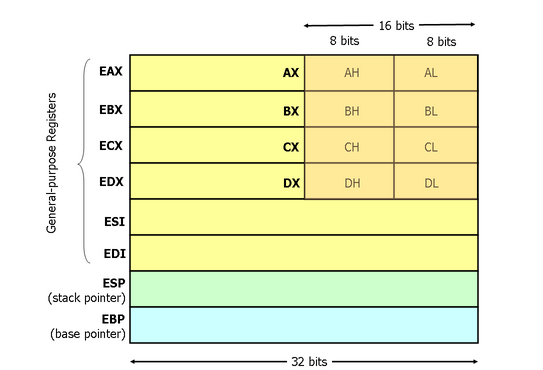
\includegraphics[width=15cm, height=9cm]{x86 Registers}
    
        x86 Registers
    
 \end{center}

 \section{Memory and Addressing Modes}

 \subsection{Declaring Static Data Regions}

 You can declare static data regions in x86 assembly using special assembler directives for this purpose.
 Data declarations should be preceded by the .DATA directive. Following this directive, the directives DB, DW, and DD
 can be used to declare one, two and four byte daha locations, respectively. \\

 Example declarations:

 \begin{center}

    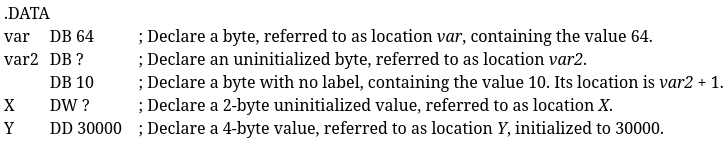
\includegraphics[width=12cm, height=2cm]{dec}

    
 \end{center}

 Unlike in high level languages where arrays can have many dimensions and are accessed by indices, arrays in x86 assembly language are simply a number of cells located 
 contiguously in memory. An array can be declared by just listing the values, as in the example below.Two other common methods used for declaring arrays of data are the DUP directive and the use of string literals. The DUP directive tells the assembler to duplicate an expression a given number of times. For example, 4 DUP(2) is equivalent to 2, 2, 2, 2. 

 \begin{center}

    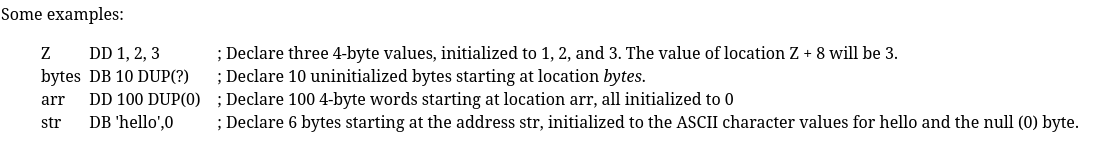
\includegraphics[width=12cm, height=2cm]{dec1}

    
 \end{center}

 \subsection{Addressing Memory}

 Modern x86-compatible processors are capable of addressing up to 232 bytes of memory: memory addresses are 32-bits wide. In the examples above, where we used labels to refer to memory regions, these labels are actually replaced by the assembler with 32-bit quantities that specify addresses in memory. In addition to supporting referring to memory regions by labels (i.e. constant values), the x86 provides a flexible scheme for computing and referring to memory addresses: up to two of the 32-bit registers and a 32-bit signed constant can be added together to compute a memory address. One of the registers can be optionally pre-multiplied by 2, 4, or 8.

The addressing nodes can be used with many x86 instructions. Here is examples using the mov instruction that moves data between registers and memory. This instruction has two operands.

\begin{center}

    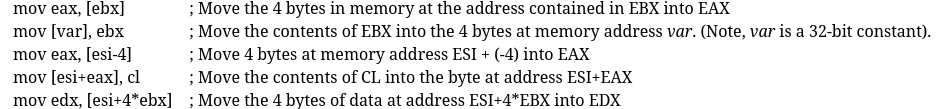
\includegraphics[width=12cm, height=2cm]{dec2}

    
 \end{center}

 \section{Instructions}

 Machine instructions generally fall into three categories: data movement, arithmetic/logic, and control-flow. Look at important examples of 
 x86 instructions from each category. Some of useful subset. for the complete list you might look at Intel's instruction set reference.

 \begin{center}

    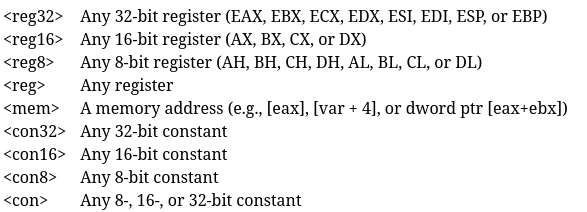
\includegraphics[width=12cm, height=4cm]{dec3}
    
 \end{center}

 \subsection{Data Movement Instructions}

 mov - Move(OPcodes: 88,89, 8A, 8B, 8C, 8E ..) \\

 The mov instruction copies the data item referred to by its second operand (i.e. register contents, memory contents, or a constant value) into the location referred to by its first operand (i.e. a register or memory). While register-to-register moves are possible, direct memory-to-memory moves are not. In cases where memory transfers are desired, the source memory contents must first be loaded into a register, then can be stored to the destination memory address.

 \begin{center}

    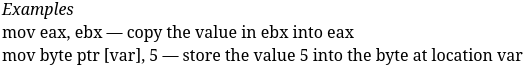
\includegraphics[width=12cm, height=1.5cm]{dec4}
    
 \end{center}

 push - Push stack(OPcodes: FF, 89, 8A, 8B, 8C, 8E, ...) \\

 The push instruction places its operand onto the top of the hardware supported stack in memory. Specifically, push first decrements ESP by 4, then places its operand into the contents of the 32-bit location at address [ESP]. ESP (the stack pointer) is decremented by push since the x86 stack grows down, the stack grows from high addresses to lower addresses. 

 \begin{center}

    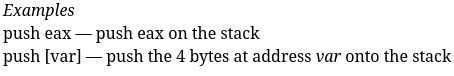
\includegraphics[width=12cm, height=1.5cm]{dec5}
    
 \end{center}

 pop - Pop stack \\

 The pop instruction removes the 4-byte data element from the top of the hardware-supported stack into the specified operand (i.e. register or memory location). It first moves the 4 bytes located at memory location [SP] into the specified register or memory location, and then increments SP by 4. 

\begin{center}

    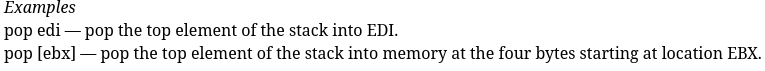
\includegraphics[width=12cm, height=1.5cm]{pop}
    
 \end{center}

 lea -- Load effective address \\

 The lea instruction places the address specified by its second operand into the register specified by its first operand. Note, the contents of the memory location are not loaded, only the effective address is computed and placed into the register. This is useful for obtaining a pointer into a memory region.

 \begin{center}

    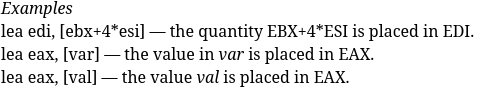
\includegraphics[width=12cm, height=1.5cm]{lea}
    
 \end{center}

 \subsection{Arithmetic and Logic Instructions}

 add - Integer Addition \\

 The add instruction adds together its two operands, storing the result in its first operand. Note, whereas both operands may be registers, at most one operand may be a memory location. 

\begin{center}

    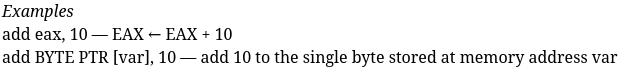
\includegraphics[width=10cm, height=1.5cm]{add}
    
 \end{center}

 sub - Integer Subtraction \\

 The sub instruction stores in the value of its first operand the result of subtracting the value of its second operand from the value of its first operand. As with add.

 \begin{center}

    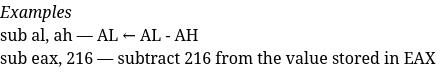
\includegraphics[width=10cm, height=1.5cm]{sub}
    
 \end{center}

 inc, dec - Increment, Decrement \\ 

 The inc instruction increments the contents of its operand by one. The dec instruction decrements the contents of its operand by one.

 \begin{center}

    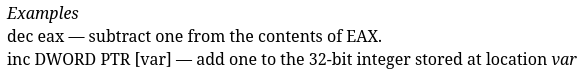
\includegraphics[width=10cm, height=1.5cm]{inc-dec}
    
 \end{center}

 imul - Integer Multiplication \\

 The imul instruction has two basic formats: two-operand (first two syntax listings above) and three-operand (last two syntax listings above).

The two-operand form multiplies its two operands together and stores the result in the first operand. The result (i.e. first) operand must be a register.  \\


 \begin{center}

    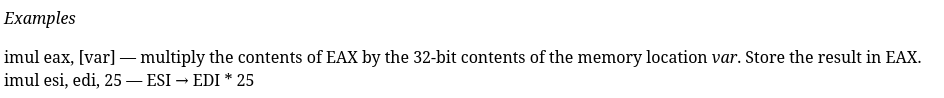
\includegraphics[width=13cm, height=1.5cm]{imul}
    
 \end{center}

 idiv - Integer Division \\ 

 The idiv instruction divides the contents of the 64 bit integer EDX:EAX (constructed by viewing EDX as the most significant four bytes and EAX as the least significant four bytes) by the specified operand value. The quotient result of the division is stored into EAX, while the remainder is placed in EDX. 

 \begin{center}

    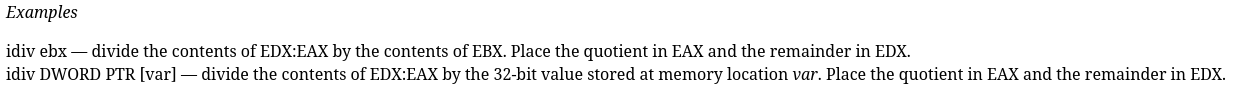
\includegraphics[width=16cm, height=2cm]{idiv}
    
 \end{center}

 and, or, xor - Bitwise logical and, or and exclusive or //

 These instructions perform the specified logical operation (logical bitwise and, or, and exclusive or, respectively) on their operands, placing the result in the first operand location. 

 \begin{center}

    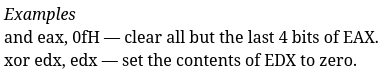
\includegraphics[width=8cm, height=2cm]{andd}
    
 \end{center}

 not - Bitwise Logical Not \\ 

 Logically negates the operand contents

 \begin{center}

    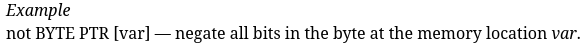
\includegraphics[width=11cm, height=1cm]{not}
    
 \end{center}

 neg - Negate \\

 Performs the two's complement negation of the operand contents.

 \begin{center}

    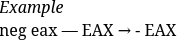
\includegraphics[width=5cm, height=0.9cm]{neg}
    
 \end{center}

 sh1, shr - Shift Left, Shift Right \\ 

 These instructions shift the bits in their first operand's contents left and right, padding the resulting empty bit positions with zeros. The shifted operand can be shifted up to 31 places. The number of bits to shift is specified by the second operand, which can be either an 8-bit constant or the register CL. In either case, shifts counts of greater then 31 are performed modulo 32. 

 \begin{center}

    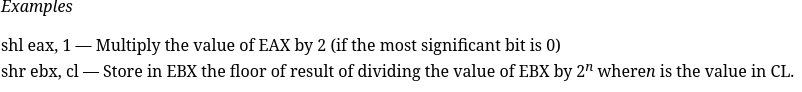
\includegraphics[width=11cm, height=1.4cm]{sh}
    
 \end{center}

 \subsection{Control Flow Instructions}

 The x86 processor maintains an instruction pointer (IP) register that is a 32-bit value indicating the location in memory where the current instruction starts. Normally, it increments to point to the next instruction in memory begins after execution an instruction. The IP register cannot be manipulated directly, but is updated implicitly by provided control flow instructions. 
 \\ We use the notation label to refer to labeled locations in the program text. Labels can be inserted anywhere in x86 assembly code text by entering a label name followed by a colon.

\begin{center}
mov esi, [ebp+8]\\
begin: xor ecx, ecx\\
mov eax, [esi]\\
\end{center}

The second instruction in this code fragment is labeled begin. Elsewhere in the code, we can refer to the memory location that this instruction is located at in memory using the more convenient symbolic name begin. This label is just a convenient way of expressing the location instead of its 32-bit value.
\\
\\\\
jmp - Jump \\

Transfers program control flow to the instruction at the memory location indicated by the operand.

\begin{center}
    jmp begin — Jump to the instruction labeled begin. 
\end{center}

jcondition - Conditional Jump \\

These instructions are conditional jumps that are based on the status of a set of condition codes that are stored in a special register called the machine status word. The contents of the machine status word include information about the last arithmetic operation performed. For example, one bit of this word indicates if the last result was zero. Another indicates if the last result was negative. Based on these condition codes, a number of conditional jumps can be performed. For example, the jz instruction performs a jump to the specified operand label if the result of the last arithmetic operation was zero. Otherwise, control proceeds to the next instruction in sequence. 

\begin{center}
    cmp eax, ebx \\
    jle done \\
    If the contents of EAX are less than or equal to the contents of EBX, jump to the label done. Otherwise, continue to the next instruction. 

\end{center}

cmp - Compare \\

Compare the values of the two specified operands, setting the condition codes in the machine status word appropriately. This instruction is equivalent to the sub instruction, except the result of the subtraction is discarded instead of replacing the first operand. 

\begin{center}
    cmp DWORD PTR [var], 10 \\
jeq loop
\end{center}

call,ret - Subroutine call and return \\

If the 4 bytes stored at location var are equal to the 4-byte integer constant 10, jump to the location labeled loop. 

These instructions implement a subroutine call and return. The call instruction first pushes the current code location onto the hardware supported stack in memory (see the push instruction for details), and then performs an unconditional jump to the code location indicated by the label operand. Unlike the simple jump instructions, the call instruction saves the location to return to when the subroutine completes. 

The ret instruction implements a subroutine return mechanism. This instruction first pops a code location off the hardware supported in-memory stack. It then performs an unconditional jump to the retrieved code location. 


\section{Creating a  MASM Assembly Program}

In Visual Studio we can start like this:

\subsection{Create a clean Project}

File | New | Project \\
Expand the ‘Other Project Types‘ tree, Select ‘Visual Studio Solutions‘, and create a new ‘Blank Solution‘.

\begin{center}

    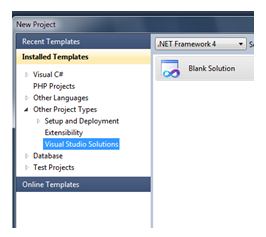
\includegraphics[width=11cm, height=4cm]{tt}
    
 \end{center}
 \newpage 
File | Add | New Project

Expand the ‘Other Languages‘, ‘Visual C++‘, ‘General‘ section and create a new ‘Empty Project‘

\begin{center}

    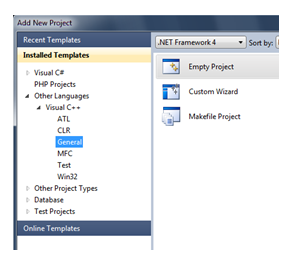
\includegraphics[width=11cm, height=4cm]{tt1}
    
 \end{center}

 \subsection{Acquire the MASM options}

 Now right click on the Project in the Solution Explorer and select ‘Build Customizations.
 \begin{center}

    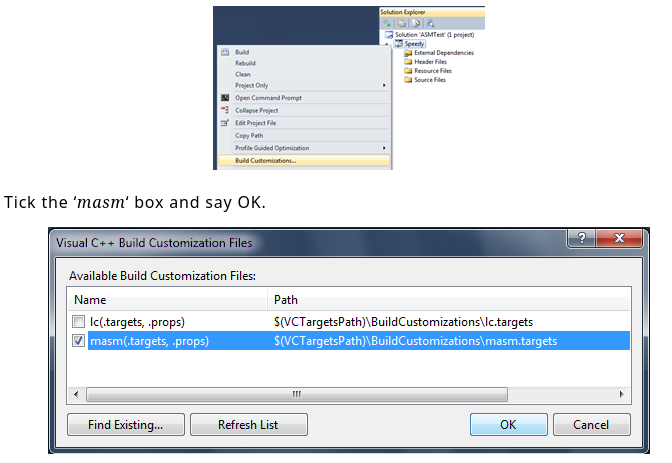
\includegraphics[width=11cm, height=7cm]{tt2}
    
 \end{center}

 Add a new file to the project with the .asm extension by right clicking on the Project in the Solution Explorer and selecting ‘Add | New Item…‘ then ‘Text File‘. Enter a filename ending with .asm (e.g. speedy.asm). Say OK.

 \begin{center}

    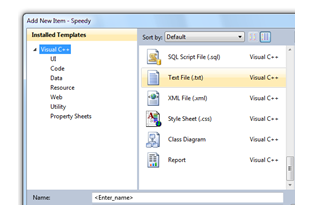
\includegraphics[width=11cm, height=7cm]{tty}
    
 \end{center}

 Now (and if you skipped the last steps this won’t work) right click on the Project and select ‘Properties‘. You should see a dialog like this (Note the MASM item at the bottom of the tree). If you don’t then something went wrong.

 \begin{center}

    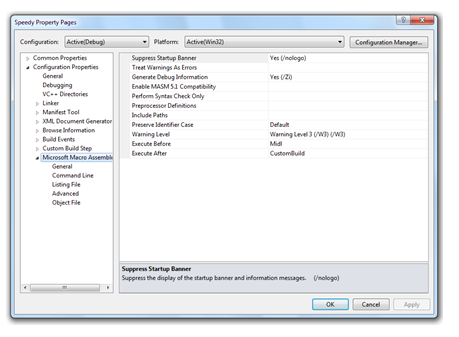
\includegraphics[width=11cm, height=7cm]{yy}
    
 \end{center}

 \subsection{Configure the linker}

 There are a few critical things to set up in the Linker options in order to get it to work:

Set the following property to Windows or Console as appropriate

Configuration Properties | Linker | System | SubSystem

\begin{center}

    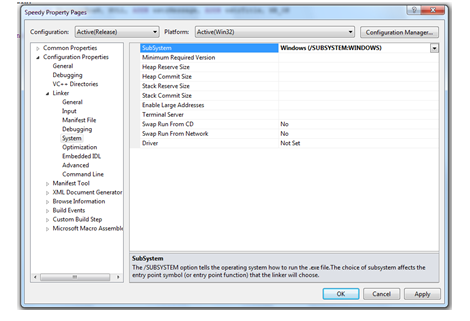
\includegraphics[width=11cm, height=7cm]{12}
    
 \end{center}

 Set the entry point to the name of your main method (as per the END directive – see code)

Configuration Properties | Linker | Advanced | EntryPoint

\begin{center}

    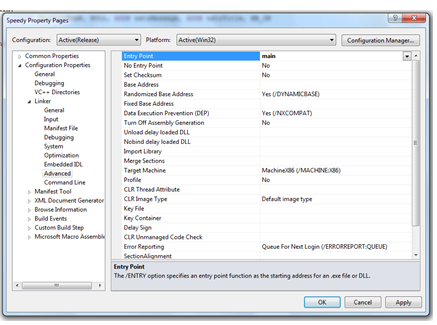
\includegraphics[width=11cm, height=7cm]{13}
    
 \end{center}

 \subsection{How to write code and execute it?}

 \begin{center}

    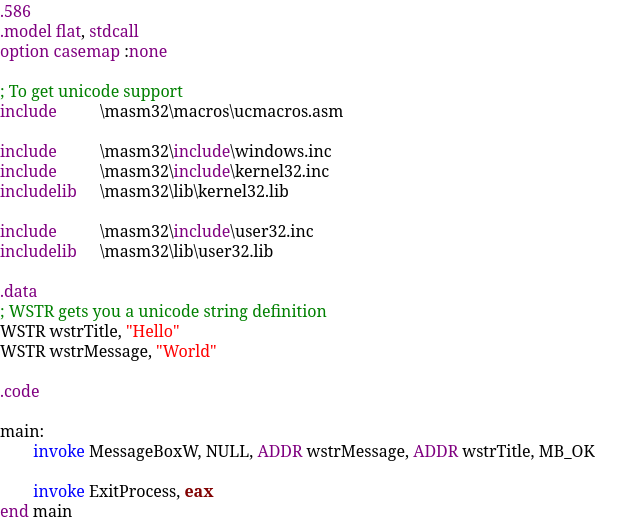
\includegraphics[width=11cm, height=7cm]{code}
    
 \end{center}

 Important thing to note here is the "end main" directive. This directive must be present and the name must match the label where you expect execution to kick off and the ‘EntryPoint’ we defined in step 3. Otherwise things simply won’t work.

 CTRL + SHIFT + B to build and run so its gonna show a simple windows message box.


 









\section{References}

\begin{itemize}
    \item Guide to Using Assembly in Visual Studio - a tutorial on building and debugging assembly code in Visual Studio.
    \item Intel x86 Instruction Set References
\end{itemize}
8. Describe 32-bit Assembler of Microsoft, worked under Windows. Give an example for creating, compiling,linking and executing of a program.
















\end{document}